\chapter{Priors, Posteriors and Conjugacy}
\label{ch:bayes-intro}

\begin{chaptergoals}
\begin{itemize}[nosep]
\item The Bayesian model: a prior distribution for the parameter, the statistical model read as the distribution of the data given the parameter, and the posterior that Bayes' formula makes from the two. Computed first on a grid of nine values of the kiss proportion.
\item Conjugate priors, which keep the posterior in the prior's family: Beta for a proportion, Gamma for a rate, Gaussian for a mean. The kiss data, the subway waits and the wind turbine, and the prior read as extra observations.
\item Updating one observation at a time, and why it gives the same posterior as all the data at once.
\item Summaries of the posterior: the posterior mean, which is best under squared error, the median, the mode, and the probability that the next couple turns right.
\item Probabilities of intervals and of hypotheses: with a flat prior they come close to confidence levels and one-sided $p$-values while answering a different question, and a point null gets a very different number. The Bernstein--von Mises theorem: with enough data the prior stops mattering, and the posterior is the Gaussian of \cref{ch:mle-properties}.
\end{itemize}
\Cref{ch:ks} ended the book's tests, all of which treated the parameter as a fixed unknown number. This chapter gives it a distribution.
\end{chaptergoals}

\section{A distribution for the parameter}
\label{sec:bayes-why}

Every chapter so far has treated $p$, the proportion of couples who turn their heads to the right, as a fixed unknown number.
The data are random and $p$ is not, so every conclusion has been a statement about a procedure: an interval that covers $p$ in $95\%$ of repetitions, a test that rejects a true null $5\%$ of the time.
\Cref{ch:confidence-intervals} named the statement most people want instead, `the probability that $p$ is between $0.56$ and $0.73$ is $0.95$', and noted that it needs $p$ to have a distribution.

The Bayesian approach gives it one.
Before the data, what is known about $p$ is described by a probability distribution, the \textbf{prior}; after the data, by the conditional distribution of $p$ given the data, the \textbf{posterior}.
The model for the data is the one used all along, now read as the distribution of the data given $p$.
Nothing here claims that $p$ is random in the world: the couples have whatever preference they have.
The distribution describes knowledge about $p$, and the data change the knowledge.
That is the difference \cref{ch:kiss} promised, and the rest of the chapter computes with it.

A prior can be read in three ways, and the mathematics is the same for all of them.
As a degree of belief: someone who is $90\%$ sure that $p$ lies between $0.4$ and $0.6$ can write that down as a distribution, and the rules of probability are what keep such beliefs consistent (if someone's betting odds break those rules, a bookmaker can choose bets against them that win whatever happens: the Dutch book argument).
As a state of information: what was known before the study, from earlier studies or from constraints such as $0 \leq p \leq 1$.
As a device: a way to build estimators, which are then judged by the criteria of \cref{ch:estimators} like any others.

\begin{bridge}[Bayes' rule]
An introductory course states Bayes' rule for two events, often with a medical test: the probability of the disease given a positive test is the probability of a positive test given the disease, times the prevalence, divided by the overall probability of a positive test.
The formula of this chapter is the same rule with `the parameter equals $\theta$' in place of the disease and the observed data in place of the positive test.
The prevalence becomes the prior, the test's accuracy becomes the likelihood, and the answer is the posterior.
The denominator, the overall chance of what was observed, adds the numerator up over every value the parameter could take.
\end{bridge}

\section{Bayes' formula for a parameter}
\label{sec:bayes-formula}

Start with a parameter that can take only finitely many values, where the rule is the one for events.
Suppose that before the kiss study $p$ was thought equally likely to be any of $0.1, 0.2, \ldots, 0.9$: prior probability $\frac19$ each.
A sequence of $124$ outcomes with $80$ right turns has probability $p^{80}(1 - p)^{44}$ under each candidate (the probability of exactly $80$ right turns in any order adds a binomial coefficient, the same for every candidate, which cancels).
Bayes' rule multiplies each prior probability by this likelihood and divides by the sum over the nine candidates:
\[
\Pr(p = 0.6 \mid \text{data}) = \frac{\frac19 \cdot 0.6^{80}\,0.4^{44}}{\sum_{j=1}^9 \frac19 (j/10)^{80}(1 - j/10)^{44}} = 0.58.
\]
The prior probabilities cancel, since they are equal, and what remains is the likelihood at $0.6$ as a share of its sum over the grid.
In natural frequencies: picture $900{,}000$ repetitions of the study, $100{,}000$ for each candidate.
Of the $100{,}000$ with $p = 0.6$, about $4{,}378$ see exactly $80$ right turns; of those with $p = 0.7$, about $3{,}160$; with $p = 0.5$, about $37$; with $p = 0.8$, about $2$; with the other five values, essentially none.
Among the roughly $7{,}580$ repetitions that saw what was seen, $58\%$ had $p = 0.6$, $42\%$ had $p = 0.7$, and half a percent had $p = \frac12$.
That is the posterior, drawn in \cref{fig:bayesgrid}: the likelihood decides which candidates survive, and the prior, flat here, decides nothing.

\begin{figure}[htbp]
\centering
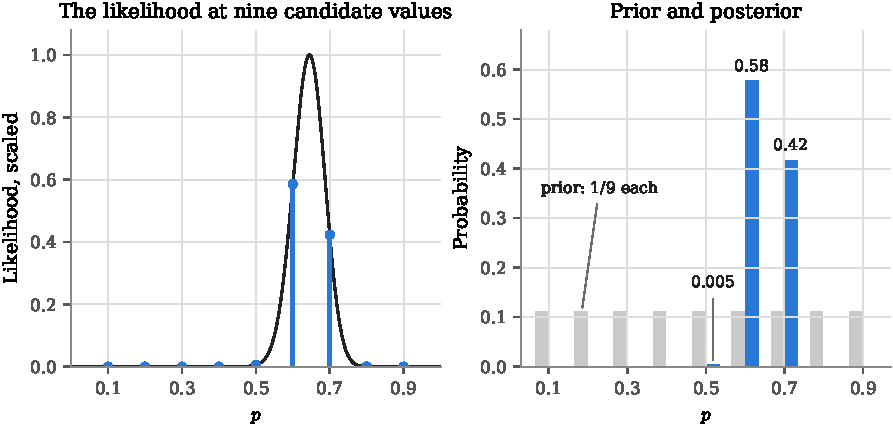
\includegraphics[width=\textwidth]{fig_bayes_grid}
\caption{The kiss data and a prior of $\frac19$ on each of $p = 0.1, 0.2, \ldots, 0.9$. Left: the likelihood $p^{80}(1 - p)^{44}$ scaled to maximum $1$ (black) and its values at the nine candidates (blue). Right: prior (gray) and posterior (blue).}
\label{fig:bayesgrid}
\end{figure}

For a parameter that varies continuously, sums become integrals.

\begin{definition}[Prior and posterior]
\label{def:posterior}
Let $(E, (\Pr_\theta)_{\theta \in \Theta})$ be a statistical model for $\Xton$ with likelihood $L_n(x_1, \ldots, x_n; \theta)$ (\cref{def:likelihood-discrete,def:likelihood-continuous}), and write $\mathbf{x} = (x_1, \ldots, x_n)$. A \textbf{prior} is a probability distribution on $\Theta$ with density $\pi$, or with PMF $\pi$ when $\Theta$ is finite or countable (this $\pi$ is unrelated to the mixture weight of \cref{ch:models,ch:likelihood}). The \textbf{Bayesian model} takes $\theta$ random with distribution $\pi$ and, given $\theta$, the observations i.i.d.\ $\Pr_\theta$. The \textbf{posterior} is the conditional distribution of $\theta$ given $X_1 = x_1, \ldots, X_n = x_n$, with density (or PMF)
\[
\pi(\theta \mid \mathbf{x}) = \frac{L_n(\mathbf{x}; \theta)\,\pi(\theta)}{m(\mathbf{x})}, \qquad m(\mathbf{x}) = \int_\Theta L_n(\mathbf{x}; t)\,\pi(t)\,\mathrm{d}t,
\]
defined whenever $0 < m(\mathbf{x}) < \infty$, with a sum in place of the integral when $\Theta$ is finite or countable. The denominator $m(\mathbf{x})$ is the \textbf{marginal likelihood} of the data.
\end{definition}

\begin{inwords}
\textbf{In words.} Posterior is likelihood times prior, rescaled to total probability $1$. Both are read as functions of $\theta$ with the data held fixed, and the marginal likelihood is the rescaling constant: the probability, or density, that the model and the prior together gave the data before they were seen.
\par\smallskip
\textbf{For the kiss data.} The likelihood is $L_n = p^{80}(1 - p)^{44}$, and with the flat prior $\pi(p) = 1$ on $(0, 1)$ the posterior density is $p^{80}(1 - p)^{44}/m$, where $m = \int_0^1 t^{80}(1 - t)^{44}\,\mathrm{d}t$. It is the black curve on the left of \cref{fig:bayesgrid}, rescaled to be a density.
\end{inwords}

The condition $0 < m(\mathbf{x}) < \infty$ rules out two things: data that every allowed $\theta$ calls impossible, where $m(\mathbf{x}) = 0$, and a likelihood so large over some values of $\theta$ that the integral diverges, which cannot happen for discrete data, since then $L_n \leq 1$ and so $m(\mathbf{x}) \leq 1$.
The condition holds in every example of this chapter.
The formula is the definition of a conditional density.
The joint density of the parameter and the data is $\pi(\theta)L_n(\mathbf{x}; \theta)$, the density of $\theta$ times the density of the data given $\theta$; the density of the data alone is this joint density integrated over $\theta$, which is $m(\mathbf{x})$; and a conditional density is a joint density divided by the density of what is conditioned on, the continuous version of $\Pr(A \mid B) = \Pr(A \cap B)/\Pr(B)$.
The same formula covers four cases: a parameter that is discrete or continuous, and data that are discrete or continuous.
For discrete data $L_n$ is a product of PMFs and for continuous data a product of densities; for a discrete parameter $m$ is a sum over $\Theta$ and for a continuous one an integral. (With discrete data and a continuous parameter the joint distribution is a PMF in the data and a density in $\theta$.)

Since $m(\mathbf{x})$ does not depend on $\theta$, it never needs computing to find the shape of the posterior.
A nonnegative function with a finite, nonzero integral is proportional to exactly one density, so it is enough to compute $L_n(\mathbf{x}; \theta)\pi(\theta)$, drop every factor that does not involve $\theta$, and recognize what is left.
The symbol $\propto$, `is proportional to as a function of $\theta$', records this:
\[
\pi(\theta \mid \mathbf{x}) \propto L_n(\mathbf{x}; \theta)\,\pi(\theta).
\]

\begin{pitfall}[a prior of zero cannot be undone]
Where $\pi(\theta) = 0$, the product $L_n\pi$ is $0$, so the posterior is $0$ there whatever the data say.
In the grid of \cref{fig:bayesgrid}, the value $0.645$ had prior probability $0$, and the posterior puts nearly all its weight on its two neighbors, $0.6$ and $0.7$.
A prior uniform on $[0.3, 0.8]$ would rule out every $p$ above $0.8$ for good, even if every couple turned right.
A prior should give some probability to every value that is not impossible.
\end{pitfall}

\section{The Beta prior for a proportion}
\label{sec:bayes-beta}

A grid works, but a family of densities on $(0, 1)$ that matches the shape of the likelihood does better.

\begin{definition}[The Beta distribution]
\label{def:beta}
For $a, b > 0$, the \textbf{Beta distribution} $\Betad(a, b)$ has density
\[
f(p) = \frac{p^{a-1}(1 - p)^{b-1}}{B(a, b)}, \qquad 0 < p < 1, \qquad B(a, b) = \int_0^1 t^{a-1}(1 - t)^{b-1}\,\mathrm{d}t = \frac{\Gamma(a)\Gamma(b)}{\Gamma(a + b)},
\]
where $\Gamma(a) = \int_0^\infty t^{a-1}e^{-t}\,\mathrm{d}t$, so that $\Gamma(k) = (k - 1)!$ for $k = 1, 2, 3, \ldots$. Its mean is $a/(a + b)$, its variance $ab/\big((a + b)^2(a + b + 1)\big)$, and, when $a, b > 1$, its mode is $(a - 1)/(a + b - 2)$ (\cref{ex:bayes-beta-moments}). $\Betad(1, 1)$ is $\Unif(0, 1)$.
\end{definition}

\begin{inwords}
\textbf{In words.} A flexible family on $(0, 1)$: a larger $a$ pulls the mass toward $1$, a larger $b$ toward $0$, and $a + b$ sets how concentrated it is.
\par\smallskip
\textbf{For the kiss data.} $\Betad(1, 1)$ is the flat prior. $\Betad(33, 33)$ has mean $\frac12$ and puts $90\%$ of its probability between $0.4$ and $0.6$: the prior of a skeptic who doubts a strong preference either way.
\end{inwords}

\begin{theorem}[Beta prior, Bernoulli data]
\label{thm:beta-bernoulli}
Let $p \sim \Betad(a, b)$ and, given $p$, let $\Xton$ be i.i.d.\ $\Bern(p)$, with $S = \sum_i X_i$. The posterior is $\Betad(a + S, b + n - S)$.
\end{theorem}

\coreproof{Multiply the prior by the likelihood and keep only what depends on $p$: what is left has the shape of a Beta density, with each exponent raised by a count.}
\begin{proof}
By \cref{def:posterior},
\[
\pi(p \mid \mathbf{x}) \propto p^S(1 - p)^{n - S} \cdot \frac{p^{a-1}(1 - p)^{b-1}}{B(a, b)} \propto p^{a + S - 1}(1 - p)^{b + n - S - 1}, \qquad 0 < p < 1.
\]
Up to a constant this is the $\Betad(a + S, b + n - S)$ density, and since both integrate to $1$ the constant is $1$.
\end{proof}

\begin{intuition}[the prior as imaginary couples]
The parameters tell the story: updating adds the $S$ right turns to $a$ and the $n - S$ left turns to $b$, so in the posterior $a$ and $b$ play the part of right and left turns seen before the study.
The posterior mean is
\[
\frac{a + S}{a + b + n} = w\,\frac{a}{a + b} + (1 - w)\,\frac{S}{n}, \qquad w = \frac{a + b}{a + b + n},
\]
a weighted average of the prior mean and the sample proportion, with the prior weighted by its $a + b$ imaginary couples against the $n$ real ones.
For the kiss data the flat prior counts as $2$ imaginary couples in the posterior mean (its density, $p^0(1 - p)^0$, adds nothing to the likelihood), weight $w = 2/126 = 0.016$, and the posterior mean is $81/126 = 0.643$; $\Betad(10, 10)$ is $20$ couples, $w = 0.139$, mean $90/144 = 0.625$; the skeptic's $\Betad(33, 33)$ is $66$ couples, $w = 0.347$, mean $113/190 = 0.595$.
As $n$ grows with the prior fixed, $w$ falls like $1/n$.
\end{intuition}

\Cref{fig:bayesbeta} draws the three priors and their posteriors.
The flat prior's posterior, $\Betad(81, 45)$, is the likelihood made into a density, with standard deviation $0.043$.
The skeptic's posterior, $\Betad(113, 77)$, is pulled a third of the way back toward $\frac12$, yet even the skeptic now puts probability $0.996$ on $p > \frac12$. The $124$ couples persuade someone who started $90\%$ sure that any preference was weak that couples do prefer the right, though not that the preference is strong: the skeptic still puts $0.56$ on $p < 0.6$.

\begin{figure}[htbp]
\centering
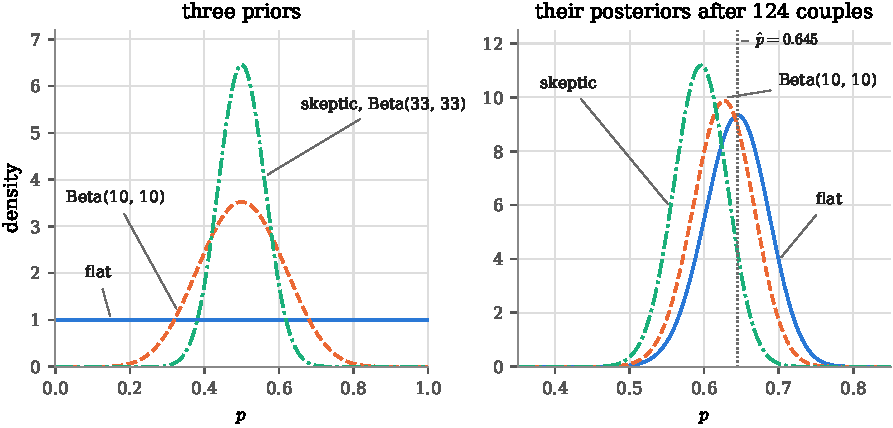
\includegraphics[width=\textwidth]{fig_bayes_beta}
\caption{Left: the priors $\Betad(1, 1)$ (blue), $\Betad(10, 10)$ (orange, dashed) and the skeptic's $\Betad(33, 33)$ (aqua, dash-dot). Right: their posteriors after $80$ right turns among $124$ couples, and $\hat{p} = 0.645$ (dotted).}
\label{fig:bayesbeta}
\end{figure}

The shrinkage estimator $(n\bar{R}_n + 10)/(n + 20)$ of \cref{sec:est-risk}, which pulled the estimate toward $\frac12$ `as if $20$ extra coin flips had come up half heads', is the posterior mean under the $\Betad(10, 10)$ prior: $90/144 = 0.625$ for the kiss data.
The imaginary flips are the prior's $a + b = 20$ couples.
\Cref{ch:estimators} found that it has lower risk than $\bar{R}_n$ when $p$ is near $\frac12$ and higher risk far from it, which in Bayesian terms says that it does best where its prior puts the weight.

\begin{bridge}[the plus-four estimate]
The plus-four interval of \cref{sec:ci-coverage}, taught in some introductory courses, adds two successes and two failures and is centered at $\tilde{p} = (S + 2)/(n + 4)$ in place of $\hat{p}$.
The estimate $\tilde{p}$ is the posterior mean under the $\Betad(2, 2)$ prior. For the kiss data it is $82/128 = 0.641$.
\end{bridge}

\begin{definition}[Conjugate prior]
\label{def:conjugate}
A family of priors is \textbf{conjugate} for a statistical model if, for every prior in the family and every sample, the posterior is again in the family.
\end{definition}

\begin{inwords}
\textbf{In words.} With a conjugate prior, updating changes the parameters of the prior and nothing else, so the posterior is a formula instead of an integral to compute.
\par\smallskip
\textbf{For the kiss data.} The Beta family is conjugate for Bernoulli data (\cref{thm:beta-bernoulli}): updating adds the number of right turns to $a$ and the number of left turns to $b$.
\end{inwords}

\begin{sanitycheck}[Where must the posterior mean land?]
Between the prior mean and the sample proportion, by the weighted average above, and closer to whichever stands for more couples.
A posterior mean outside $[0.5, 0.645]$ for a prior with mean $\frac12$ and the kiss data signals an arithmetic error.
The skeptic's $0.595$ passes: $0.347 \times 0.5 + 0.653 \times 0.645 = 0.595$.
\end{sanitycheck}

\section{Rates and means: two more conjugate pairs}
\label{sec:bayes-conjugate}

A rate can be any positive number and a mean any real number, so neither fits a prior on $(0, 1)$.
For a rate the conjugate family is the Gamma.

\begin{definition}[The Gamma distribution]
\label{def:gamma}
For $\alpha, \beta > 0$, the \textbf{Gamma distribution} $\Gammad(\alpha, \beta)$, with shape $\alpha$ and rate $\beta$, has density
\[
f(\lambda) = \frac{\beta^\alpha\lambda^{\alpha - 1}e^{-\beta\lambda}}{\Gamma(\alpha)}, \qquad \lambda > 0,
\]
with mean $\alpha/\beta$ and variance $\alpha/\beta^2$. $\Gammad(1, \beta)$ is $\Expo(\beta)$.
\end{definition}

\begin{inwords}
\textbf{In words.} A flexible family on $(0, \infty)$, the natural home for a rate. Its mean $\alpha/\beta$ reads as $\alpha$ events in a time $\beta$.
\par\smallskip
\textbf{For the kiss data.} The kiss proportion lives in $(0, 1)$, so its prior is a Beta, not a Gamma; the Gamma is for the subway rate $\lambda$, trains per minute, which can be any positive number.
\end{inwords}

\begin{proposition}[Gamma prior, exponential data]
\label{prop:gamma-expo}
Let $\lambda \sim \Gammad(\alpha, \beta)$ and, given $\lambda$, let $T_1, \ldots, T_n$ be i.i.d.\ $\Expo(\lambda)$. The posterior is $\Gammad\big(\alpha + n, \beta + \sum_i T_i\big)$.
\end{proposition}

\optionalproof{The same recognition as for the Beta: the likelihood $\lambda^n e^{-\lambda\sum T_i}$ has the shape of a Gamma density in $\lambda$.}
\begin{proof}
$\pi(\lambda \mid \mathbf{t}) \propto \lambda^n e^{-\lambda\sum_i t_i} \cdot \lambda^{\alpha - 1}e^{-\beta\lambda} = \lambda^{\alpha + n - 1}e^{-(\beta + \sum_i t_i)\lambda}$ for $\lambda > 0$, the shape of the $\Gammad(\alpha + n, \beta + \sum_i t_i)$ density.
\end{proof}

In the posterior's parameters the prior again acts as imaginary data, here $\alpha$ waits lasting $\beta$ minutes in total.
For the subway, suppose the timetable promises a train every $5$ minutes, and take a prior with mean $0.2$ trains per minute that counts as $30$ waits: $\Gammad(30, 150)$.
The $64$ observed waits total $64 \times 6.23 = 398.7$ minutes, so the posterior is $\Gammad(94, 548.7)$, with mean $94/548.7 = 0.171$ and standard deviation $\sqrt{94}/548.7 = 0.018$.
The maximum likelihood estimate is $1/6.23 = 0.161$. The reciprocal of the posterior mean, $548.7/94 = 5.84$ minutes per train, is the average of the timetable's $5$ and the observed $6.23$, weighted by $30$ imaginary waits and $64$ real ones.

\begin{proposition}[Gaussian prior, Gaussian data with known variance]
\label{prop:normal-normal}
Let $\mu \sim \Gauss(\mu_0, \sigma_0^2)$ and, given $\mu$, let $\Xton$ be i.i.d.\ $\Gauss(\mu, \sigma^2)$ with $\sigma^2$ known. The posterior is $\Gauss(\mu_n, \sigma_n^2)$ with
\[
\frac{1}{\sigma_n^2} = \frac{1}{\sigma_0^2} + \frac{n}{\sigma^2}, \qquad \mu_n = \sigma_n^2\Big(\frac{\mu_0}{\sigma_0^2} + \frac{n\bar{x}_n}{\sigma^2}\Big).
\]
\end{proposition}

\optionalproof{Multiply the two Gaussian shapes; the exponent is a quadratic in $\mu$, and completing the square names its center and spread.}
\begin{proof}
Using $\sum_i(x_i - \mu)^2 = \sum_i(x_i - \bar{x}_n)^2 + n(\bar{x}_n - \mu)^2$ and dropping factors free of $\mu$,
\[
\pi(\mu \mid \mathbf{x}) \propto \exp\Big(-\frac{n(\mu - \bar{x}_n)^2}{2\sigma^2} - \frac{(\mu - \mu_0)^2}{2\sigma_0^2}\Big) \propto \exp\Big(-\frac{\mu^2}{2}\Big(\frac{n}{\sigma^2} + \frac{1}{\sigma_0^2}\Big) + \mu\Big(\frac{n\bar{x}_n}{\sigma^2} + \frac{\mu_0}{\sigma_0^2}\Big)\Big).
\]
Since $-\frac{\mu^2}{2\sigma_n^2} + \frac{\mu\mu_n}{\sigma_n^2} = -\frac{(\mu - \mu_n)^2}{2\sigma_n^2} + \frac{\mu_n^2}{2\sigma_n^2}$, the last expression is proportional to $\exp\big(-(\mu - \mu_n)^2/(2\sigma_n^2)\big)$, the shape of the $\Gauss(\mu_n, \sigma_n^2)$ density.
\end{proof}

The reciprocal of a variance is a \textbf{precision}, and the proposition says that precisions add: the prior contributes $1/\sigma_0^2$, each observation $1/\sigma^2$, and the posterior mean is the average of $\mu_0$ and $\bar{x}_n$ weighted by their precisions.
The prior counts as $\sigma^2/\sigma_0^2$ observations.
The same calculation works when the observations have different known variances $\sigma_i^2$: each $x_i$ is weighted by $1/\sigma_i^2$, and the prior mean enters as one more observation with variance $\sigma_0^2$.

\Cref{ch:t-test} asked whether the mean wind speed $\mu$ at a home is above $10$ miles per hour, from $12$ monthly measurements with mean $14.3$ and standard deviation $4.7$.
Take $\sigma = 4.7$ as known, and a prior centered at $11$, a regional average, with standard deviation $2$.
The prior counts as $4.7^2/2^2 = 5.5$ months of data, so the posterior mean is $(5.5 \times 11 + 12 \times 14.3)/17.5 = 13.26$ and the posterior standard deviation is $4.7/\sqrt{17.5} = 1.12$.
Where the $t$-test of \cref{ch:t-test} rejected $\mu \leq 10$, the posterior gives a probability: $\Pr(\mu > 10 \mid \text{data}) = 1 - \Phi\big((10 - 13.26)/1.12\big) = 0.998$.
(Treating $\sigma$ as unknown needs a prior for $\sigma$ too. With $\sigma$ independent of $\mu$ and a prior density proportional to $1/\sigma$, a common choice that \cref{ch:jeffreys} explains, the probability is $0.991$. That density has an infinite integral, so it is not a probability distribution and \cref{def:posterior} does not cover it; \cref{ch:jeffreys} says why the posterior is still a proper distribution.)
\Cref{fig:bayesconj} draws both examples, and in both the posterior lies between the prior and the likelihood and is narrower than either; on the right, the area under the posterior to the right of the gray line at $10$ is the $0.998$ above.

\begin{figure}[htbp]
\centering
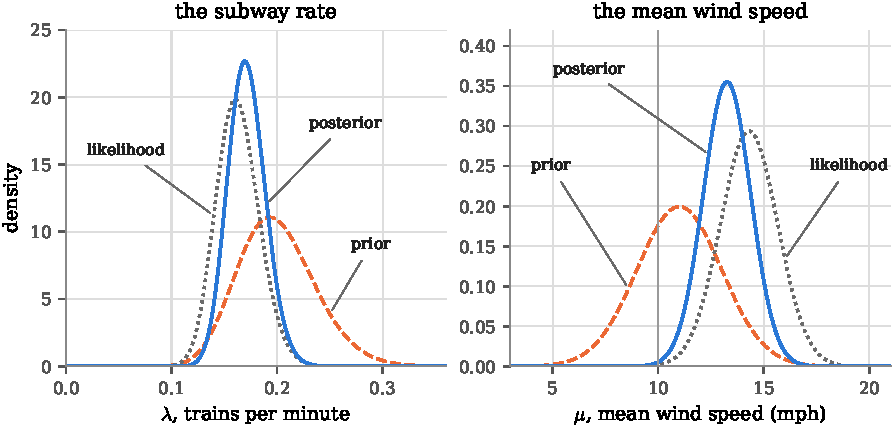
\includegraphics[width=\textwidth]{fig_bayes_conjugate}
\caption{Prior (orange, dashed), likelihood scaled to a density (gray, dotted) and posterior (blue). Left: the subway rate, prior $\Gammad(30, 150)$, posterior $\Gammad(94, 548.7)$. Right: the mean wind speed, prior $\Gauss(11, 2^2)$, posterior $\Gauss(13.26, 1.12^2)$; gray line at $10$.}
\label{fig:bayesconj}
\end{figure}

\begin{center}
\small
\begin{tabular}{@{}lll@{}}
\toprule
model for the data & conjugate prior & posterior \\
\midrule
$\Bern(p)$ & $p \sim \Betad(a, b)$ & $\Betad\big(a + \sum X_i, b + n - \sum X_i\big)$ \\
$\Pois(\lambda)$ & $\lambda \sim \Gammad(\alpha, \beta)$ & $\Gammad\big(\alpha + \sum X_i, \beta + n\big)$ (\cref{ex:bayes-siblings}) \\
$\Expo(\lambda)$ & $\lambda \sim \Gammad(\alpha, \beta)$ & $\Gammad\big(\alpha + n, \beta + \sum X_i\big)$ \\
$\Gauss(\mu, \sigma^2)$, $\sigma^2$ known & $\mu \sim \Gauss(\mu_0, \sigma_0^2)$ & $\Gauss(\mu_n, \sigma_n^2)$ of \cref{prop:normal-normal} \\
$\Gauss(0, v)$ & $v \sim$ Inverse Gamma$(a, b)$ & Inverse Gamma$\big(a + \frac{n}{2}, b + \frac12\sum X_i^2\big)$ (\cref{ex:bayes-invgamma}) \\
\bottomrule
\end{tabular}
\end{center}

(The Inverse Gamma is the distribution of $1/V$ for $V \sim \Gammad(a, b)$.)
Without a conjugate prior the posterior is still defined by the same formula, and only the computation changes.
With one or two parameters a grid like \cref{fig:bayesgrid} with a fine mesh is enough.
With many parameters the posterior is explored by simulating draws from it, with methods called Markov chain Monte Carlo, which are beyond this book.

\section{One observation at a time}
\label{sec:bayes-sequential}

Does it matter whether the data arrive all at once or one couple at a time?
It does not.

\begin{proposition}[Updating in stages]
\label{prop:bayes-stages}
For data i.i.d.\ given $\theta$ and any $m < n$, the posterior given $x_1, \ldots, x_n$ is the posterior obtained by using $\pi(\theta \mid x_1, \ldots, x_m)$ as the prior and $x_{m+1}, \ldots, x_n$ as the data.
\end{proposition}

\optionalproof{The likelihood of all the data is the product of the likelihoods of the two batches.}
\begin{proof}
$L_n(x_1, \ldots, x_n; \theta) = L_m(x_1, \ldots, x_m; \theta)\,L_{n-m}(x_{m+1}, \ldots, x_n; \theta)$ (\cref{ch:likelihood}), so
\begin{align*}
\pi(\theta \mid x_1, \ldots, x_n) &\propto L_{n-m}(x_{m+1}, \ldots, x_n; \theta)\,\big[L_m(x_1, \ldots, x_m; \theta)\,\pi(\theta)\big] \\
&\propto L_{n-m}(x_{m+1}, \ldots, x_n; \theta)\,\pi(\theta \mid x_1, \ldots, x_m). \qedhere
\end{align*}
\end{proof}

Yesterday's posterior is today's prior. Applying the proposition repeatedly feeds the data in one observation at a time, and the order does not matter, since the likelihood is a product of one factor per observation.
\Cref{fig:bayessequential} does it for the kiss data with the flat prior, with the $124$ outcomes in a random order, since the study does not report the order.
The first couple turned left, and the posterior $\Betad(1, 2)$ already has mean $\frac13$; after $10$ couples, $5$ of them right, the posterior mean is $\frac12$ and the middle $95\%$ of the posterior runs from $0.23$ to $0.77$; after $40$ couples it runs from $0.42$ to $0.72$, and after all $124$ from $0.558$ to $0.724$, which is the solve interval of \cref{ch:confidence-intervals} to three decimals (\cref{sec:bayes-bvm} explains why the two nearly agree).
Early on, each couple moves the posterior visibly; by the end, a single couple moves the mean by $0.003$ if it turns right and by $0.005$ if it turns left.

\begin{figure}[htbp]
\centering
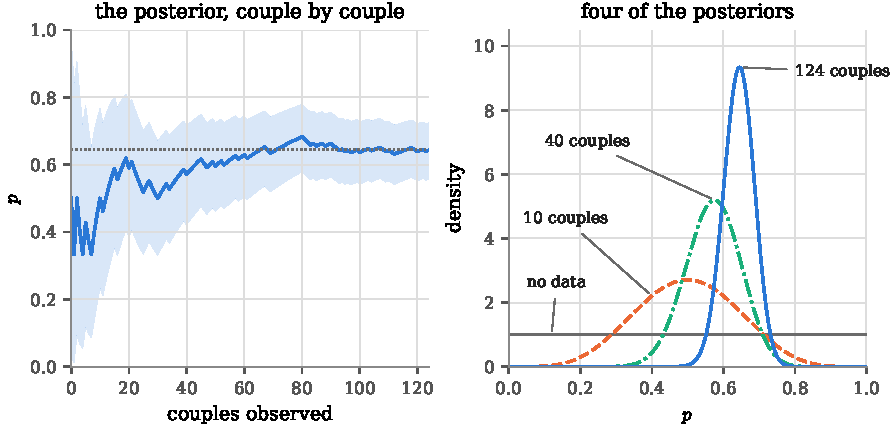
\includegraphics[width=\textwidth]{fig_bayes_sequential}
\caption{Kiss data, one couple at a time, flat prior. Left: posterior mean (blue), middle $95\%$ (shaded), $0.645$ (dotted). Right: posteriors after $0$ (gray), $10$ (orange, dashed), $40$ (aqua, dash-dot) and $124$ (blue) couples.}
\label{fig:bayessequential}
\end{figure}

\section{Summarizing the posterior}
\label{sec:bayes-summaries}

The posterior is the whole answer, and a report still needs numbers.
Three of them describe where it sits.

\begin{definition}[Posterior mean, median and mode]
\label{def:bayes-estimators}
The \textbf{posterior mean} $\E[\theta \mid \mathbf{x}] = \int_\Theta \theta\,\pi(\theta \mid \mathbf{x})\,\mathrm{d}\theta$ is also called the \textbf{Bayes estimator} for squared error. The \textbf{posterior median} is a median of the posterior distribution. The \textbf{maximum a posteriori} (MAP) estimate is a value of $\theta$ that maximizes $\pi(\theta \mid \mathbf{x})$, the mode of the posterior.
\end{definition}

\begin{inwords}
\textbf{In words.} The center of mass, the halfway point and the peak of the posterior. For a symmetric posterior with one peak they coincide; for a skewed one they spread out, usually in the order mode, median, mean, toward the long tail.
\par\smallskip
\textbf{For the kiss data.} With the flat prior the posterior is $\Betad(81, 45)$: mean $81/126 = 0.643$, median $0.644$, mode $80/124 = 0.645$, which is $\hat{p}$.
\end{inwords}

Why the mean?
Because it is the best single number under squared error, by the same identity as the bias--variance decomposition of \cref{ch:estimators}.

\begin{proposition}[The posterior mean minimizes squared error]
\label{prop:posterior-mean}
For a posterior with finite variance and every number $c$,
\[
\E\big[(\theta - c)^2 \mid \mathbf{x}\big] = \var(\theta \mid \mathbf{x}) + \big(\E[\theta \mid \mathbf{x}] - c\big)^2.
\]
So the posterior mean minimizes the posterior expected squared error, and the minimum is the posterior variance.
\end{proposition}

\optionalproof{The bias--variance identity of \cref{thm:bias-variance}, with the posterior in place of the sampling distribution and $c$ in place of the true value: the cross term averages to zero.}
\begin{proof}
Write $\bar\theta = \E[\theta \mid \mathbf{x}]$. Then $(\theta - c)^2 = (\theta - \bar\theta)^2 + 2(\theta - \bar\theta)(\bar\theta - c) + (\bar\theta - c)^2$. Take the posterior expectation of each term: the first gives $\var(\theta \mid \mathbf{x})$; in the second, $\bar\theta - c$ is a number and $\E[\theta - \bar\theta \mid \mathbf{x}] = 0$; the third is a number. The first term does not involve $c$, and the last is smallest, $0$, at $c = \bar\theta$.
\end{proof}

The same reasoning with absolute error picks the posterior median: \cref{prop:median-min}, applied to the posterior distribution, says the median minimizes $\E[\abs{\theta - c} \mid \mathbf{x}]$ (its hypotheses, a continuous density with a finite mean, hold for the Beta posteriors with both parameters above $1$ and for the Gamma and Gaussian posteriors here).
The mode answers a different question.
Taking logarithms,
\[
\log\pi(\theta \mid \mathbf{x}) = \ell_n(\theta) + \log\pi(\theta) - \log m(\mathbf{x}),
\]
so the MAP estimate maximizes the log-likelihood plus $\log\pi(\theta)$, which is very negative where the prior is small and so works as a penalty.
With a flat prior the penalty is constant and the MAP estimate is the maximum likelihood estimator; with a Gaussian prior $\Gauss(\mu_0, \sigma_0^2)$ it is $-(\theta - \mu_0)^2/(2\sigma_0^2)$ plus a constant, a quadratic penalty that pulls toward $\mu_0$ (in regression the same penalty is called ridge).

\begin{pitfall}[the MAP estimate depends on the parameterization]
The maximum likelihood estimator follows any one-to-one change of parameter (\cref{prop:mle-invariance}); the MAP estimate does not: a density changes shape when its variable is transformed. If $\psi = g(p)$ with $g$ increasing, then $\Pr(\psi \leq t) = \Pr(p \leq g^{-1}(t))$, and differentiating in $t$ shows that the density of $\psi$ is the density of $p$ times $\mathrm{d}p/\mathrm{d}\psi$.
With the flat prior, the MAP estimate of $p$ for the kiss data is $0.645$.
The log-odds $\psi = \log\big(p/(1 - p)\big)$ has posterior density $\pi(p \mid \mathbf{x})\,p(1 - p) \propto p^{81}(1 - p)^{45}$, written in terms of $p$, which peaks at $p = 81/126 = 0.643$ (\cref{ex:bayes-map}).
The two MAP estimates describe different values of $p$.
The posterior median follows every increasing change of parameter, since it is defined by probabilities.
\end{pitfall}

The posterior also predicts.
The probability that the next couple turns right, given the data, averages $p$ over the posterior:
\[
\Pr(X_{n+1} = 1 \mid \mathbf{x}) = \int_0^1 p\,\pi(p \mid \mathbf{x})\,\mathrm{d}p = \E[p \mid \mathbf{x}] = \frac{a + S}{a + b + n}.
\]
With the flat prior this is $(S + 1)/(n + 2)$, Laplace's rule of succession: $81/126 = 0.643$ for the kiss data, close to the plug-in $\hat{p} = 0.645$.
The two differ when data are few: after $3$ right turns in $3$ couples the plug-in answer is $1$, a certainty that a fourth will turn right, and Laplace's rule gives $0.8$.
Laplace's $0.8$ is the plug-in $1$ pulled toward the prior mean $\frac12$ by the two imaginary couples: $0.8 = \frac25 \times \frac12 + \frac35 \times 1$.

\section{Probabilities of intervals and of hypotheses}
\label{sec:bayes-hypotheses}

\Cref{ch:confidence-intervals} called `$\Pr(p \in [0.56, 0.73]) = 0.95$' a Bayesian statement and said this chapter would say what it costs.
The posterior gives such probabilities directly.
For the kiss data, $\Pr(0.56 \leq p \leq 0.73 \mid \text{data})$ is $0.955$ with the flat prior, $0.941$ with $\Betad(10, 10)$ and $0.835$ with the skeptic's prior.
The cost is the prior: the probability belongs to the prior and the data together, and a reader with a different prior gets a different number.
With the flat prior it comes out near the confidence level $0.95$ ($0.952$ for the plug-in interval $[0.561, 0.729]$ itself; rounding it out to $[0.56, 0.73]$ gives $0.955$), and \cref{sec:bayes-bvm} explains why.
The question \cref{ch:likelihood} could not answer, the probability that $p$ is between $0.6$ and $0.7$, now has an answer: $0.75$ with the flat prior.

A one-sided hypothesis gets a probability the same way.
With the flat prior, $\Pr(p \leq \frac12 \mid \text{data}) = 0.0006$, the same number as the one-sided $p$-value of \cref{ch:tests-foundations} by the Gaussian approximation (the exact Binomial $p$-value is $0.0008$; \cref{ex:bayes-tail} explains the near agreement).
The numbers agree; the questions do not.
The $p$-value is the probability of data this extreme if $p = \frac12$; the posterior probability is the probability that $p \leq \frac12$ given the data.

A point hypothesis such as $H_0: p = \frac12$ is different, and \cref{ch:tests-foundations} promised a different number for it.
Under a continuous prior a single value has probability $0$, before and after the data, so a prior that takes $H_0$ seriously must put a lump of probability on $p = \frac12$.
Take probability $\frac12$ on $p = \frac12$ and spread the other $\frac12$ uniformly over $(0, 1)$.
This prior has neither a density nor a PMF, so \cref{def:posterior} does not cover it, but Bayes' rule for the two events $H_0: p = \frac12$ and $H_1: p \neq \frac12$ does.
Write $m_0$ and $m_1$ for the probability of the data under $H_0$ and under $H_1$; then $m(\mathbf{x}) = m_0\Pr(H_0) + m_1\Pr(H_1)$, $\Pr(H_j \mid \mathbf{x}) = m_j\Pr(H_j)/m(\mathbf{x})$ for $j = 0, 1$, and dividing the two gives the odds form,
\[
\frac{\Pr(H_0 \mid \mathbf{x})}{\Pr(H_1 \mid \mathbf{x})} = \frac{m_0}{m_1} \cdot \frac{\Pr(H_0)}{\Pr(H_1)},
\]
where $m_0 = 2^{-124} = 4.7 \times 10^{-38}$ and $m_1 = \int_0^1 p^{80}(1 - p)^{44}\,\mathrm{d}p = 1.0 \times 10^{-36}$, the probability of the data averaged over the uniform prior: the area under the sequence likelihood that \cref{ch:likelihood} said meant nothing as an area, and that means something here.
The ratio $B_{01} = m_0/m_1$ is the \textbf{Bayes factor}; here it is $0.0465$, the prior odds are $1$, and so $\Pr(H_0 \mid \mathbf{x}) = 0.0465/1.0465 = 0.044$.
Among $1{,}000$ studies that saw $80$ right turns, in a world where no preference and a uniformly spread preference were equally likely beforehand, about $44$ had no preference.
The two-sided $p$-value was $0.0012$, about $36$ times smaller.
The data favor a preference by a factor of $1/B_{01} = 21$; the likelihood ratio of \cref{ch:wald-lrt}, $e^{10.60/2} = 200$, is about nine times larger, since it compares $H_0$ with the single best value $\hat{p}$, while the Bayes factor compares it with the average over every $p$, including values the data rule out.

The gap grows with $n$.
Keep the two-sided $p$-value at $0.0012$, so that the standardized statistic stays $3.23$, and let the number of couples grow, with the same prior:
\begin{center}
\small
\begin{tabular}{@{}lrrrrr@{}}
\toprule
couples $n$ & $124$ & $1{,}240$ & $12{,}400$ & $124{,}000$ & $1{,}240{,}000$ \\
right turns & $80$ & $677$ & $6{,}380$ & $62{,}569$ & $621{,}800$ \\
$\Pr(H_0 \mid \text{data})$ & $0.04$ & $0.13$ & $0.32$ & $0.60$ & $0.83$ \\
\bottomrule
\end{tabular}
\end{center}
At a fixed $p$-value, a larger sample is stronger evidence for the point null, since a true preference would have produced a larger standardized statistic in a larger sample.
Lindley (\textit{Biometrika}, 1957) pointed out this divergence, now called Lindley's paradox; Berger and Sellke (\textit{Journal of the American Statistical Association}, 1987) showed that, for a Gaussian mean, at a $p$-value of $0.05$ the posterior probability of a point null with prior probability $\frac12$ is at least $0.29$ for every prior on the alternative that is symmetric about the null value with a single peak there, and at least $0.128$ for every prior whatsoever.

\section{When the data outweigh the prior}
\label{sec:bayes-bvm}

The priors of \cref{fig:bayesbeta} disagree, and their posteriors disagree less.
With more data they would disagree less still.

\recall{The Law of Large Numbers (\cref{thm:wlln}): for i.i.d.\ random variables with mean $\mu$ and finite variance, $\bar{X}_n \convp \mu$. Chebyshev's inequality \toolkit{sec:math-inequalities}: $\Pr(\abs{Y - \E[Y]} \geq t) \leq \var(Y)/t^2$ for any random variable $Y$ with finite variance and any $t > 0$.}

\begin{theorem}[The prior washes out]
\label{thm:prior-washout}
Let $a, b > 0$, and let $\Xton$ be i.i.d.\ $\Bern(p^*)$, where $p^*$ is the fixed true value. For the posterior from the prior $\Betad(a, b)$, which depends on the data and is therefore random:
\begin{enumerate}[nosep]
\item the posterior mean converges to $p^*$ in probability;
\item for every $\varepsilon > 0$, the posterior probability $\Pr(\abs{p - p^*} < \varepsilon \mid X_1, \ldots, X_n)$ converges to $1$ in probability.
\end{enumerate}
\end{theorem}

\coreproof{The weight on the prior mean is $(a + b)/(a + b + n)$, which goes to $0$, and the sample proportion goes to $p^*$; the posterior variance is at most $1/(4n)$, so the posterior piles up at its mean.}
\begin{proof}
(1) Fix $\varepsilon > 0$, let $S = \sum_i X_i$, and write $\bar{p}_n$ for the posterior mean. By the weighted average of \cref{sec:bayes-beta}, $\bar{p}_n - S/n = w_n\big(a/(a + b) - S/n\big)$ with $w_n = (a + b)/(a + b + n)$, which is at most $w_n$ in absolute value since both $a/(a + b)$ and $S/n$ lie in $[0, 1]$. So $\abs{\bar{p}_n - p^*} \leq w_n + \abs{S/n - p^*}$. Once $w_n < \varepsilon/2$, the event $\abs{\bar{p}_n - p^*} \geq \varepsilon$ forces $\abs{S/n - p^*} \geq \varepsilon/2$, whose probability tends to $0$ by the Law of Large Numbers.

(2) Write $a_n = a + S$ and $b_n = b + n - S$. The posterior variance is $a_nb_n/\big((a_n + b_n)^2(a_n + b_n + 1)\big)$, and $a_nb_n \leq (a_n + b_n)^2/4$, so it is at most $1/\big(4(a + b + n + 1)\big)$. By Chebyshev's inequality applied to the posterior distribution, the posterior probability that $p$ is at least $\varepsilon/2$ from $\bar{p}_n$ is at most $c_n = 1/\big(\varepsilon^2(a + b + n + 1)\big)$. If $p$ is within $\varepsilon/2$ of $\bar{p}_n$ and $\bar{p}_n$ is within $\varepsilon/2$ of $p^*$, then $\abs{p - p^*} < \varepsilon$. So on the event $E_n$ that $\bar{p}_n$ is within $\varepsilon/2$ of $p^*$, $Y_n = \Pr(\abs{p - p^*} < \varepsilon \mid X_1, \ldots, X_n) \geq 1 - c_n$. Given $\eta > 0$, once $c_n < \eta$ the event $Y_n \leq 1 - \eta$ lies outside $E_n$, so $\Pr(\abs{Y_n - 1} \geq \eta) \leq \Pr(E_n^c) \to 0$ by (1).
\end{proof}

\Cref{fig:bayesbvm} draws it.
At $124$ couples the three posterior means of \cref{fig:bayesbeta} spread over $0.048$, about one posterior standard deviation; with ten times as many couples in the same proportion, $800$ of $1{,}240$, they spread over $0.007$, half a standard deviation of $0.014$, and the three posteriors nearly coincide with a single Gaussian centered at $\hat{p}$ with the standard error $\sqrt{\hat{p}(1 - \hat{p})/n}$ of \cref{ch:confidence-intervals}.
That Gaussian is the general limit.

\begin{figure}[htbp]
\centering
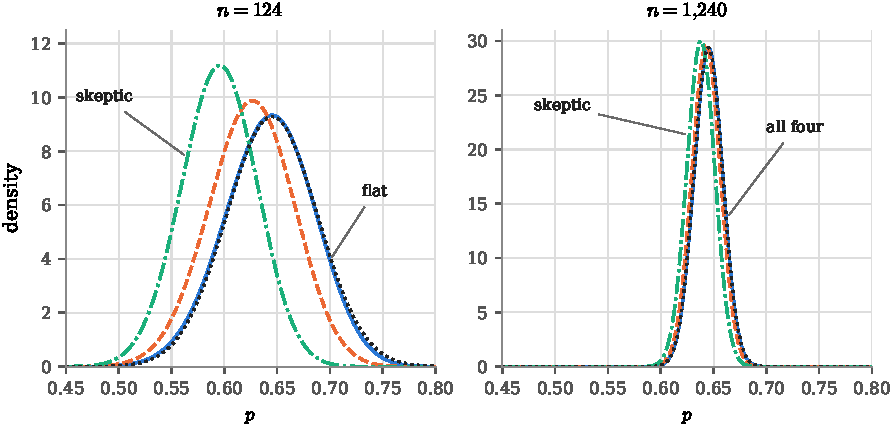
\includegraphics[width=\textwidth]{fig_bayes_bvm}
\caption{Posteriors from the flat prior (blue), $\Betad(10, 10)$ (orange, dashed) and the skeptic's $\Betad(33, 33)$ (aqua, dash-dot), with $\Gauss\big(\hat{p}, \hat{p}(1 - \hat{p})/n\big)$ (black, dotted). Left: $80$ right turns in $124$ couples. Right: $800$ in $1{,}240$.}
\label{fig:bayesbvm}
\end{figure}

\recall{Asymptotic normality of the maximum likelihood estimator (\cref{thm:mle-normal}): under the regularity conditions of \cref{sec:mle-regularity}, with $\theta^*$ in the interior of $\Theta$ and $I(\theta^*) > 0$, $\sqrt{n}(\hat{\theta}_n - \theta^*) \convd \Gauss\big(0, 1/I(\theta^*)\big)$.}

\begin{theorem}[Bernstein--von Mises]
\label{thm:bvm}
Let $\Xton \iid \Pr_{\theta^*}$ in a model satisfying the regularity conditions of \cref{sec:mle-regularity}, with $\theta^*$ in the interior of $\Theta$ and $I(\theta^*) > 0$, let $\hat{\theta}_n$ be the maximum likelihood estimator, and suppose the data separate $\theta^*$ from distant values: for every $\varepsilon > 0$ there is a $\delta > 0$ such that, with probability tending to $1$, $\frac1n\big(\ell_n(\theta) - \ell_n(\theta^*)\big) \leq -\delta$ for every $\theta$ with $\abs{\theta - \theta^*} \geq \varepsilon$ (this holds for the models of this chapter). Let the prior have a density that is continuous and positive at $\theta^*$. Then the total variation distance (\cref{ch:distances}) between the posterior distribution of $\sqrt{n}(\theta - \hat{\theta}_n)$, with $\theta$ random and $\hat{\theta}_n$ the number computed from the data, and $\Gauss\big(0, 1/I(\theta^*)\big)$ converges to $0$ in probability under $\Pr_{\theta^*}$. Informally, for large $n$ the posterior is approximately $\Gauss\big(\hat{\theta}_n, 1/(nI(\hat{\theta}_n))\big)$, for every such prior.
\end{theorem}

This theorem is stated without proof; its proof needs more than this book develops. It is named for Bernstein (1917) and von Mises (1931), though Laplace had already found it for a proportion with a flat prior; its modern form is due to Le Cam (1953).
The reason it holds is visible in the log-posterior, $\ell_n(\theta) + \log\pi(\theta)$ up to a constant.
The log-likelihood grows with $n$, and near its peak it is a parabola whose curvature is about $nI(\theta^*)$ (\cref{ch:mle-properties}); the log-prior stays the same size, and over the width of about $1/\sqrt{nI(\theta^*)}$ where the likelihood matters it is nearly constant, which is why the prior must be continuous and positive at $\theta^*$.
So for large $n$ the log-posterior is that parabola, and a density whose logarithm is a parabola is Gaussian.
\Cref{thm:mle-normal} and \cref{thm:bvm} read the same parabola from two sides: the first describes how the estimate $\hat{\theta}_n$ scatters around the fixed $\theta^*$, the second how the posterior spreads around the fixed $\hat{\theta}_n$, with the same variance $1/(nI)$.
That is why the flat-prior probability of the $95\%$ confidence interval came out near $0.95$, and why Bayesian and frequentist intervals nearly coincide in large samples.

\section{What comes next}
\label{sec:bayes-next}

Every posterior in this chapter came from a prior someone chose.
\Cref{ch:jeffreys} asks what to use when there is nothing to put in a prior: flat priors and their dependence on the parameterization, improper priors, whose density has an infinite integral and so cannot be rescaled to integrate to $1$, and Jeffreys' prior, built from the Fisher information so that it does not depend on the parameterization.
It then builds Bayesian confidence regions, intervals with a stated posterior probability, and compares them with the intervals of \cref{ch:confidence-intervals}, using the Bernstein--von Mises theorem.

\section{Summary}
\label{sec:bayes-summary}

\begin{itemize}[nosep]
\item Bayesian model: a prior $\pi$ on $\Theta$, and the data i.i.d.\ $\Pr_\theta$ given $\theta$. Posterior: $\pi(\theta \mid \mathbf{x}) \propto L_n(\mathbf{x}; \theta)\pi(\theta)$, rescaled by the marginal likelihood $m(\mathbf{x})$. A parameter value with prior probability $0$ keeps posterior probability $0$.
\item Grid: nine candidate values of the kiss proportion; the posterior puts $0.58$ on $0.6$ and $0.42$ on $0.7$.
\item Conjugate pairs: Beta prior and Bernoulli data give $\Betad(a + S, b + n - S)$; Gamma and exponential give $\Gammad(\alpha + n, \beta + \sum T_i)$; Gaussian and Gaussian give precisions that add. The prior acts as imaginary data: $a + b$ couples, $\alpha$ waits, $\sigma^2/\sigma_0^2$ observations. Kiss posterior means: $0.643$ (flat), $0.625$ ($\Betad(10, 10)$, the shrinkage estimator), $0.595$ (skeptic).
\item Updating in stages, or one observation at a time in any order, gives the same posterior.
\item Posterior mean: best under squared error, with the posterior variance as its error. Median: best under absolute error. MAP: maximizes the log-likelihood plus $\log\pi$, depends on the parameterization. The predictive probability of the next success is the posterior mean, Laplace's $(S + 1)/(n + 2)$ with a flat prior.
\item Interval and one-sided probabilities depend on the prior ($0.955$, $0.941$, $0.835$ for $[0.56, 0.73]$). A point null needs prior mass; for the kiss data its posterior probability is $0.044$ against a $p$-value of $0.0012$, and at a fixed $p$-value it grows with $n$ (Lindley).
\item The prior washes out: with Beta priors the posterior concentrates at $p^*$; in general (Bernstein--von Mises) the posterior is approximately $\Gauss\big(\hat{\theta}_n, 1/(nI(\hat{\theta}_n))\big)$.
\end{itemize}

\section{Exercises}
\label{sec:bayes-exercises}

\begin{exercise}
\label{ex:bayes-beta-moments}
Let $P \sim \Betad(a, b)$. (a) Using $B(a, b) = \Gamma(a)\Gamma(b)/\Gamma(a + b)$ and $\Gamma(x + 1) = x\Gamma(x)$, show that $\E[P] = a/(a + b)$ and $\E[P^2] = a(a + 1)/\big((a + b)(a + b + 1)\big)$, and deduce the variance. (b) Show that for $a, b > 1$ the density is largest at $(a - 1)/(a + b - 2)$.
\end{exercise}
\begin{solution}
(a) $\E[P] = \int_0^1 p \cdot p^{a-1}(1 - p)^{b-1}\,\mathrm{d}p/B(a, b) = B(a + 1, b)/B(a, b) = \frac{\Gamma(a + 1)\Gamma(a + b)}{\Gamma(a)\Gamma(a + b + 1)} = \frac{a}{a + b}$. Likewise $\E[P^2] = B(a + 2, b)/B(a, b) = \frac{a(a + 1)}{(a + b)(a + b + 1)}$. So $\var(P) = \frac{a(a + 1)}{(a + b)(a + b + 1)} - \frac{a^2}{(a + b)^2} = \frac{a\big[(a + 1)(a + b) - a(a + b + 1)\big]}{(a + b)^2(a + b + 1)} = \frac{ab}{(a + b)^2(a + b + 1)}$, since $(a + 1)(a + b) - a(a + b + 1) = b$. (b) The log-density is $(a - 1)\log p + (b - 1)\log(1 - p)$ plus a constant, with derivative $(a - 1)/p - (b - 1)/(1 - p)$, which is $0$ at $p = (a - 1)/(a + b - 2)$; the second derivative $-(a - 1)/p^2 - (b - 1)/(1 - p)^2$ is negative, so this is the maximum.
\end{solution}

\begin{exercise}
\label{ex:bayes-flat-marginal}
(a) With the flat prior on $p$, show that the number of successes $S$ in $n$ Bernoulli trials has $\Pr(S = s) = 1/(n + 1)$ for every $s = 0, 1, \ldots, n$, using $B(s + 1, n - s + 1) = s!\,(n - s)!/(n + 1)!$. (b) For the kiss data, compute $m_1 = \int_0^1 p^{80}(1 - p)^{44}\,\mathrm{d}p$ in terms of a binomial coefficient, and check the Bayes factor $B_{01} = 0.0465$ of \cref{sec:bayes-hypotheses}, given that $\binom{124}{80}2^{-124} = 0.000372$.
\end{exercise}
\begin{solution}
(a) $\Pr(S = s) = \int_0^1 \binom{n}{s}p^s(1 - p)^{n-s}\,\mathrm{d}p = \binom{n}{s}B(s + 1, n - s + 1) = \frac{n!}{s!\,(n - s)!}\cdot\frac{s!\,(n - s)!}{(n + 1)!} = \frac{1}{n + 1}$. Before any data, every count is equally likely, which is how Bayes himself chose the flat prior in 1763. (b) $m_1 = B(81, 45) = 80!\,44!/125! = 1/\big(125\binom{124}{80}\big)$, so $B_{01} = 2^{-124}/m_1 = 125\binom{124}{80}2^{-124} = 125 \times 0.000372 = 0.0465$.
\end{solution}

\begin{exercise}
\label{ex:bayes-drug}
In the drug trial of \cref{ch:kiss}, earlier studies showed the drug to be about $80\%$ effective. (a) Express this as a $\Betad(40, 10)$ prior: what is its mean, and how many patients does it count as? (b) After $78$ cures in $100$ patients, find the posterior, its mean and its standard deviation, and the weight on the prior mean. (c) Compute $\Pr(p > 0.7 \mid \text{data})$ approximately with a Gaussian approximation to the posterior.
\end{exercise}
\begin{solution}
(a) Mean $40/50 = 0.8$; it counts as $50$ patients, $40$ cured. (b) $\Betad(118, 32)$: mean $118/150 = 0.787$, standard deviation $\sqrt{118 \times 32/(150^2 \times 151)} = 0.033$; the weight on the prior mean is $50/150 = \frac13$, and $0.787 = \frac13 \times 0.8 + \frac23 \times 0.78$. (c) $\Pr(p > 0.7) \approx 1 - \Phi\big((0.7 - 0.787)/0.033\big) = 1 - \Phi(-2.6) = 0.995$ (the exact Beta value is $0.992$).
\end{solution}

\begin{exercise}
\label{ex:bayes-siblings}
(a) Show that the Gamma family is conjugate for Poisson data: if $\lambda \sim \Gammad(\alpha, \beta)$ and, given $\lambda$, $\Xton \iid \Pois(\lambda)$, the posterior is $\Gammad(\alpha + \sum_i X_i, \beta + n)$. (b) In the siblings data of \cref{ch:models}, the $24$ values of $X - 1$ add up to $24$. With the prior $\Gammad(2, 2)$, find the posterior mean and standard deviation of $\lambda$ and compare with the maximum likelihood estimate.
\end{exercise}
\begin{solution}
(a) $\pi(\lambda \mid \mathbf{x}) \propto \prod_i e^{-\lambda}\lambda^{x_i} \cdot \lambda^{\alpha - 1}e^{-\beta\lambda} = \lambda^{\alpha + \sum x_i - 1}e^{-(\beta + n)\lambda}$, the shape of $\Gammad(\alpha + \sum x_i, \beta + n)$. (b) $\Gammad(26, 26)$: mean $1.0$, standard deviation $\sqrt{26}/26 = 0.196$. The maximum likelihood estimate is the sample mean, $1.0$; the prior, with mean $1$ and worth $2$ observations, agrees with the data and only narrows the posterior.
\end{solution}

\begin{exercise}
\label{ex:bayes-geometric}
Let $X_1, \ldots, X_n$ be i.i.d.\ geometric given $p$, with $\Pr(X = x) = (1 - p)^{x-1}p$ for $x = 1, 2, \ldots$ (the trial on which the first success occurs), and let $p \sim \Betad(a, b)$. Find the posterior and the posterior mean.
\end{exercise}
\begin{solution}
$\pi(p \mid \mathbf{x}) \propto \prod_i(1 - p)^{x_i - 1}p \cdot p^{a-1}(1 - p)^{b-1} = p^{a + n - 1}(1 - p)^{b + \sum x_i - n - 1}$, so the posterior is $\Betad\big(a + n, b + \sum_i x_i - n\big)$, with mean $(a + n)/(a + b + \sum_i x_i)$. The prior again counts as data: $a$ successes and $b$ failures.
\end{solution}

\begin{exercise}
\label{ex:bayes-invgamma}
Let $\Xton \iid \Gauss(0, v)$ given $v$, and give $v$ the Inverse Gamma prior with density $\pi(v) = \frac{b^a}{\Gamma(a)}v^{-a-1}e^{-b/v}$, $v > 0$, whose mean is $b/(a - 1)$ for $a > 1$. (a) Show that the posterior is Inverse Gamma with parameters $a + n/2$ and $b + \frac12\sum_i X_i^2$. (b) Find the posterior mean and its limit as $a$ and $b$ tend to $0$ (for $n \geq 3$). Is it the maximum likelihood estimate $\frac1n\sum_i X_i^2$?
\end{exercise}
\begin{solution}
(a) $\pi(v \mid \mathbf{x}) \propto \prod_i v^{-1/2}e^{-x_i^2/(2v)} \cdot v^{-a-1}e^{-b/v} = v^{-(a + n/2) - 1}e^{-(b + \sum x_i^2/2)/v}$, the shape of the Inverse Gamma with parameters $a + n/2$ and $b + \frac12\sum_i x_i^2$. (b) The posterior mean is $\big(b + \frac12\sum_i x_i^2\big)/(a + n/2 - 1)$, which tends to $\sum_i x_i^2/(n - 2)$, not the maximum likelihood estimate $\frac1n\sum_i x_i^2$. (The posterior mode, $\big(b + \frac12\sum_i x_i^2\big)/(a + n/2 + 1)$, tends to $\sum_i x_i^2/(n + 2)$; neither summary of this posterior is the maximum likelihood estimate.)
\end{solution}

\begin{exercise}
\label{ex:bayes-tail}
(a) Show that if $S$ of $n$ trials are successes and the prior is flat, then $\Pr(p \leq x \mid \text{data}) = \Pr\big(\Bin(n + 1, x) \geq S + 1\big)$ for $0 < x < 1$. (Hint: the $(S + 1)$th smallest of $n + 1$ independent $\Unif(0, 1)$ variables has the $\Betad(S + 1, n - S + 1)$ distribution.) (b) For the kiss data, compare $\Pr(p \leq \frac12 \mid \text{data}) = \Pr(\Bin(125, \frac12) \geq 81)$ with the exact one-sided $p$-value $\Pr(\Bin(124, \frac12) \geq 80)$, which are $0.00060$ and $0.00078$.
\end{exercise}
\begin{solution}
(a) The posterior is $\Betad(S + 1, n - S + 1)$, the distribution of the $(S + 1)$th smallest of $n + 1$ independent uniforms, whose density is $\frac{(n + 1)!}{S!\,(n - S)!}u^S(1 - u)^{n - S}$. That order statistic is at most $x$ exactly when at least $S + 1$ of the $n + 1$ uniforms are at most $x$, and the number of uniforms at most $x$ is $\Bin(n + 1, x)$. (b) The posterior probability uses one more trial and one more success than the $p$-value: $\Pr(\Bin(125, \frac12) \geq 81)$ against $\Pr(\Bin(124, \frac12) \geq 80)$. The two tail probabilities are of the same size, $0.00060$ and $0.00078$, which is why the posterior probability and the one-sided $p$-value nearly agree, though they answer different questions.
\end{solution}

\begin{exercise}
\label{ex:bayes-map}
With the flat prior on $p$ and the kiss data, (a) find the posterior density of the log-odds $\psi = \log\big(p/(1 - p)\big)$, using $\mathrm{d}p/\mathrm{d}\psi = p(1 - p)$, and show that it peaks where $p = 81/126$; (b) explain why the MAP estimate of $\psi$, transformed back, is not the MAP estimate of $p$, while the posterior median of $\psi$, transformed back, is the posterior median of $p$.
\end{exercise}
\begin{solution}
(a) A density of $p$ becomes a density of $\psi$ when multiplied by $\mathrm{d}p/\mathrm{d}\psi = p(1 - p)$, so the posterior of $\psi$ is proportional to $p^{80}(1 - p)^{44}\cdot p(1 - p) = p^{81}(1 - p)^{45}$, written in terms of $p$. As $p$ increases with $\psi$, this is largest where $p^{81}(1 - p)^{45}$ is, at $p = 81/126 = 0.643$, that is $\psi = \log(81/45) = 0.588$. (b) The factor $p(1 - p)$ changes where the density peaks, so the modes of the two densities correspond to different values of $p$: $0.645$ and $0.643$. The median is defined by probabilities, $\Pr(p \leq m) = \frac12$, and an increasing map preserves them: $\Pr(\psi \leq \log(m/(1 - m))) = \Pr(p \leq m) = \frac12$.
\end{solution}

\begin{exercise}
\label{ex:bayes-predictive}
With the flat prior and the kiss data, find the probability that the next $10$ couples all turn right, $\E[p^{10} \mid \text{data}]$, as a product of $10$ fractions, and compare it with the plug-in answer $\hat{p}^{10}$.
\end{exercise}
\begin{solution}
Given $p$ the probability is $p^{10}$, so the predictive probability is $\E[p^{10} \mid \text{data}] = B(91, 45)/B(81, 45) = \prod_{j=0}^{9}\frac{81 + j}{126 + j} = 0.0145$, against $0.645^{10} = 0.0125$. By Jensen's inequality \toolkit{sec:math-convex}, $\E[p^{10} \mid \text{data}] \geq (\E[p \mid \text{data}])^{10} = 0.643^{10} = 0.0121$: values of $p$ above the mean raise $p^{10}$ more than values below it lower it. The bound alone is below $\hat{p}^{10}$, since the posterior mean is below $\hat{p}$; the exact $0.0145$ shows that the spread of the posterior adds enough to pass $\hat{p}^{10}$.
\end{solution}
